\documentclass{article}
\usepackage[utf8]{inputenc}
\usepackage[a4paper, total={6in, 8in}]{geometry}
\usepackage{graphicx}
\usepackage{minted}

\title{CS 5783 Assignment 1}
\author{Suraj Pawar}
\date{August 2019}

\begin{document}

\maketitle

\section{$k$D Tree}

\begin{figure*}[htbp]
\centering
{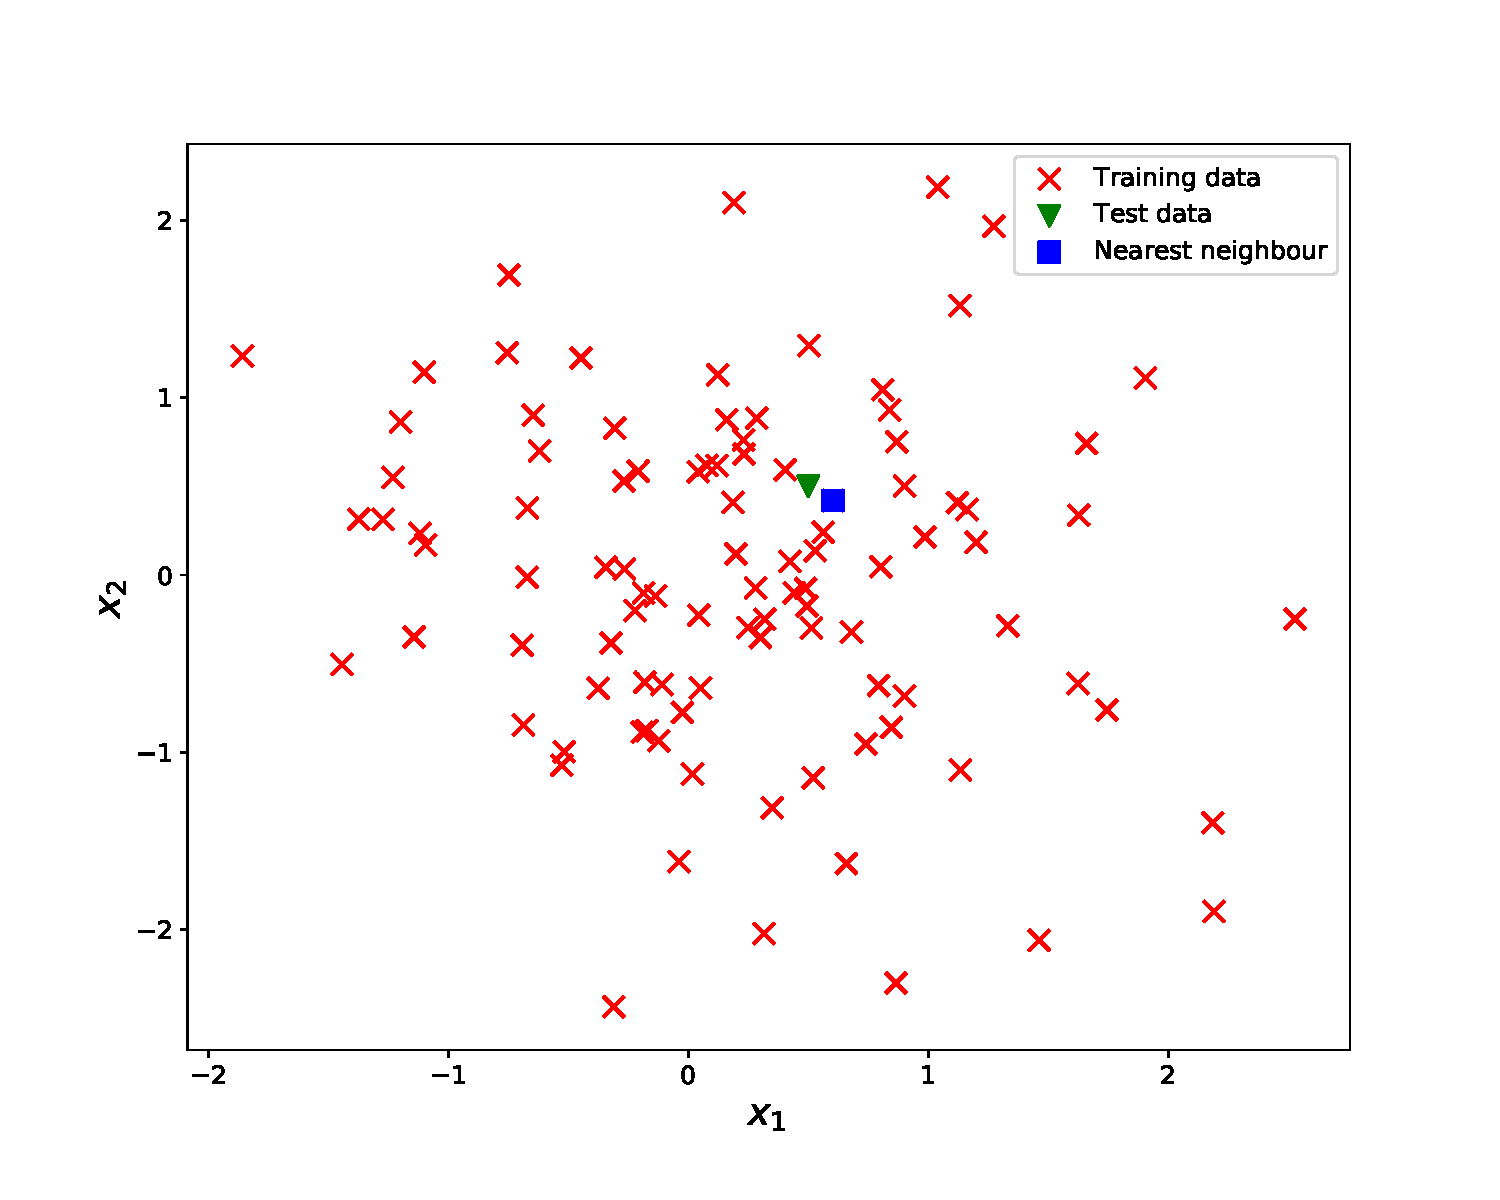
\includegraphics[width=0.8\textwidth]{figures/kdtree.pdf}}
\caption{The training data consists of 100 points selected from random normal distribution. The test data is $[0.5,0.5]$ and the nearest neighbour is correctly found.}
\label{fig:kdtree}
\end{figure*}

\newpage
\section{Constructing a simple dataset}
\begin{minted}{python}
n1 = 5000
n2 = 5000
split = 0.5

mean1 = np.random.randn(1,2).flatten()
cov1 = make_spd_matrix(2,2)
data1 = np.random.multivariate_normal(mean1, cov1, n1)
label1 = np.zeros((n1,1))

mean2 = np.random.randn(1,2).flatten()
cov2 = make_spd_matrix(2,2)
data2 = np.random.multivariate_normal(mean2, cov2, n2)
label2 = np.ones((n2,1))

data = np.vstack((data1,data2))
labels = np.vstack((label1,label2))

# select indices randomly for splitting train and test data
indices = np.full(data.shape[0],True)
indices[:int(data.shape[0]*split)] = False
np.random.shuffle(indices)

# split the data into train and test data
xtrain, ytrain = data[indices==True], labels[indices==True]
xtest, ytest = data[indices==False], labels[indices==False]
\end{minted}

\newpage
\section{Linear classifier}
\begin{figure*}[htbp]
\centering
{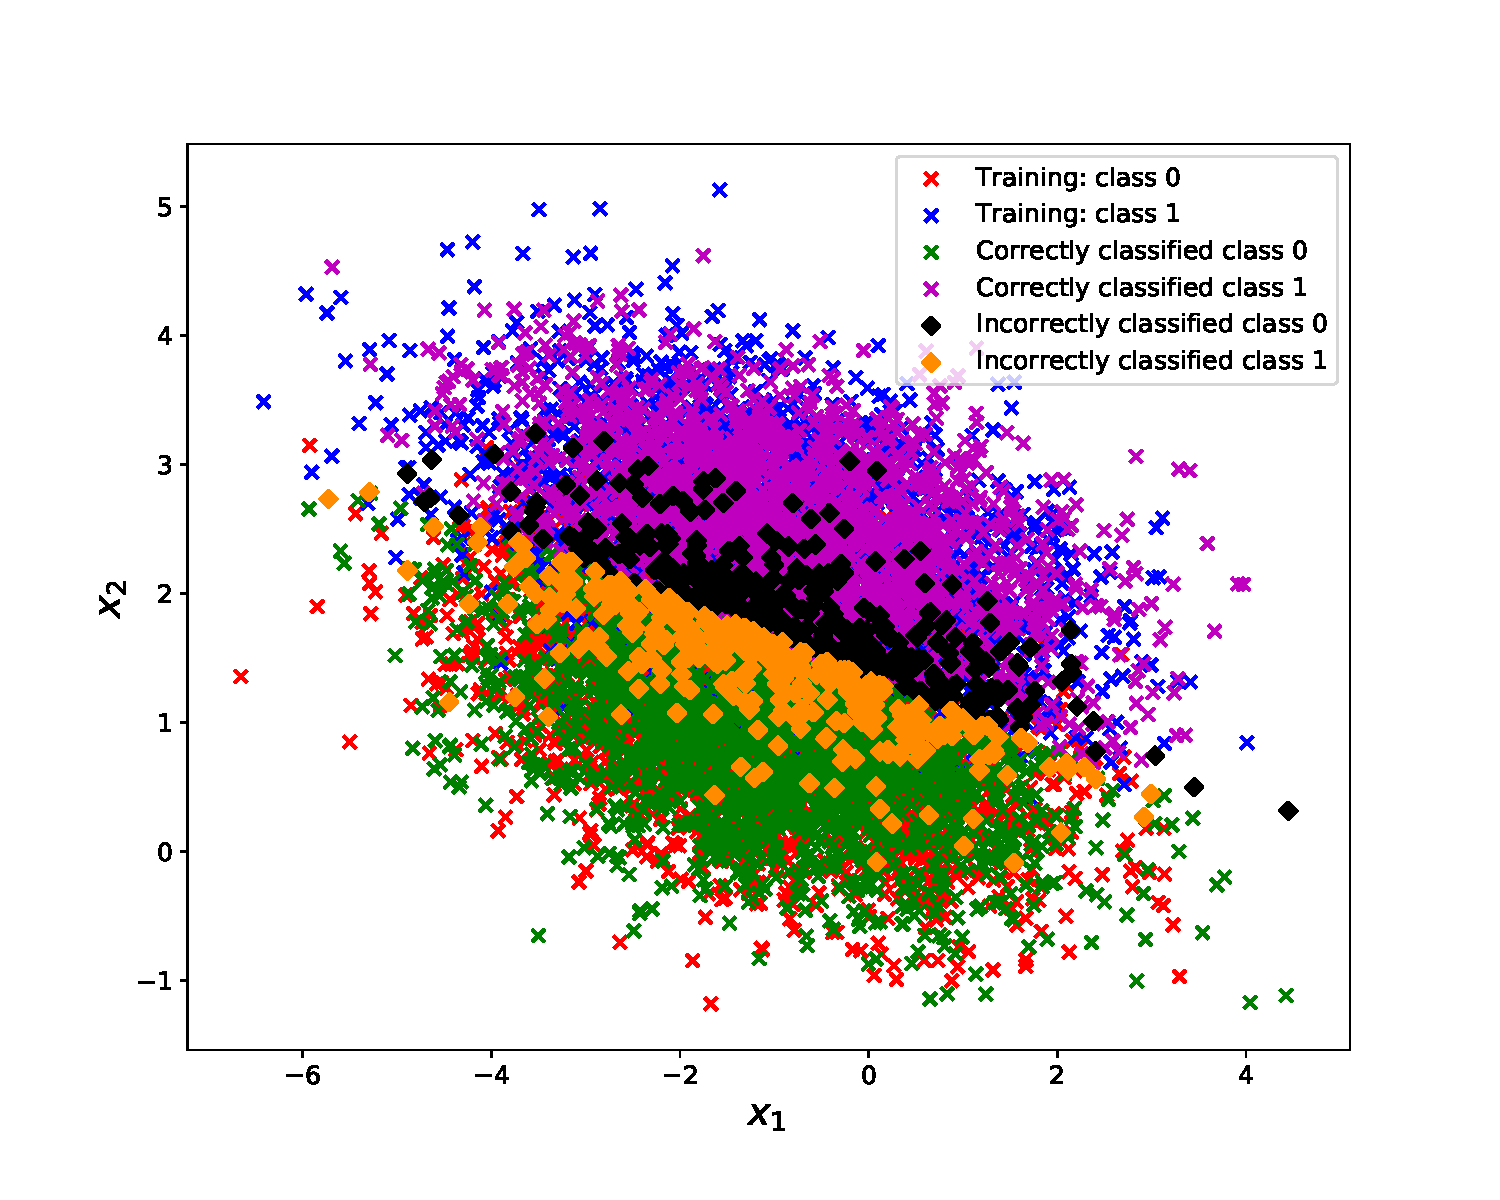
\includegraphics[width=0.8\textwidth]{figures/linear_classifier.pdf}}
\caption{The data is generated from two different multivariate Gaussian distribution and is split into train and test data with 50\%. Linear classifier achieves accuracy of \underline{\textbf{86.76\%}} on test data.}
\label{fig:lin_classifier_1}
\end{figure*}

\newpage
\section{Nearest neighbour classification}
\begin{figure*}[htbp]
\centering
{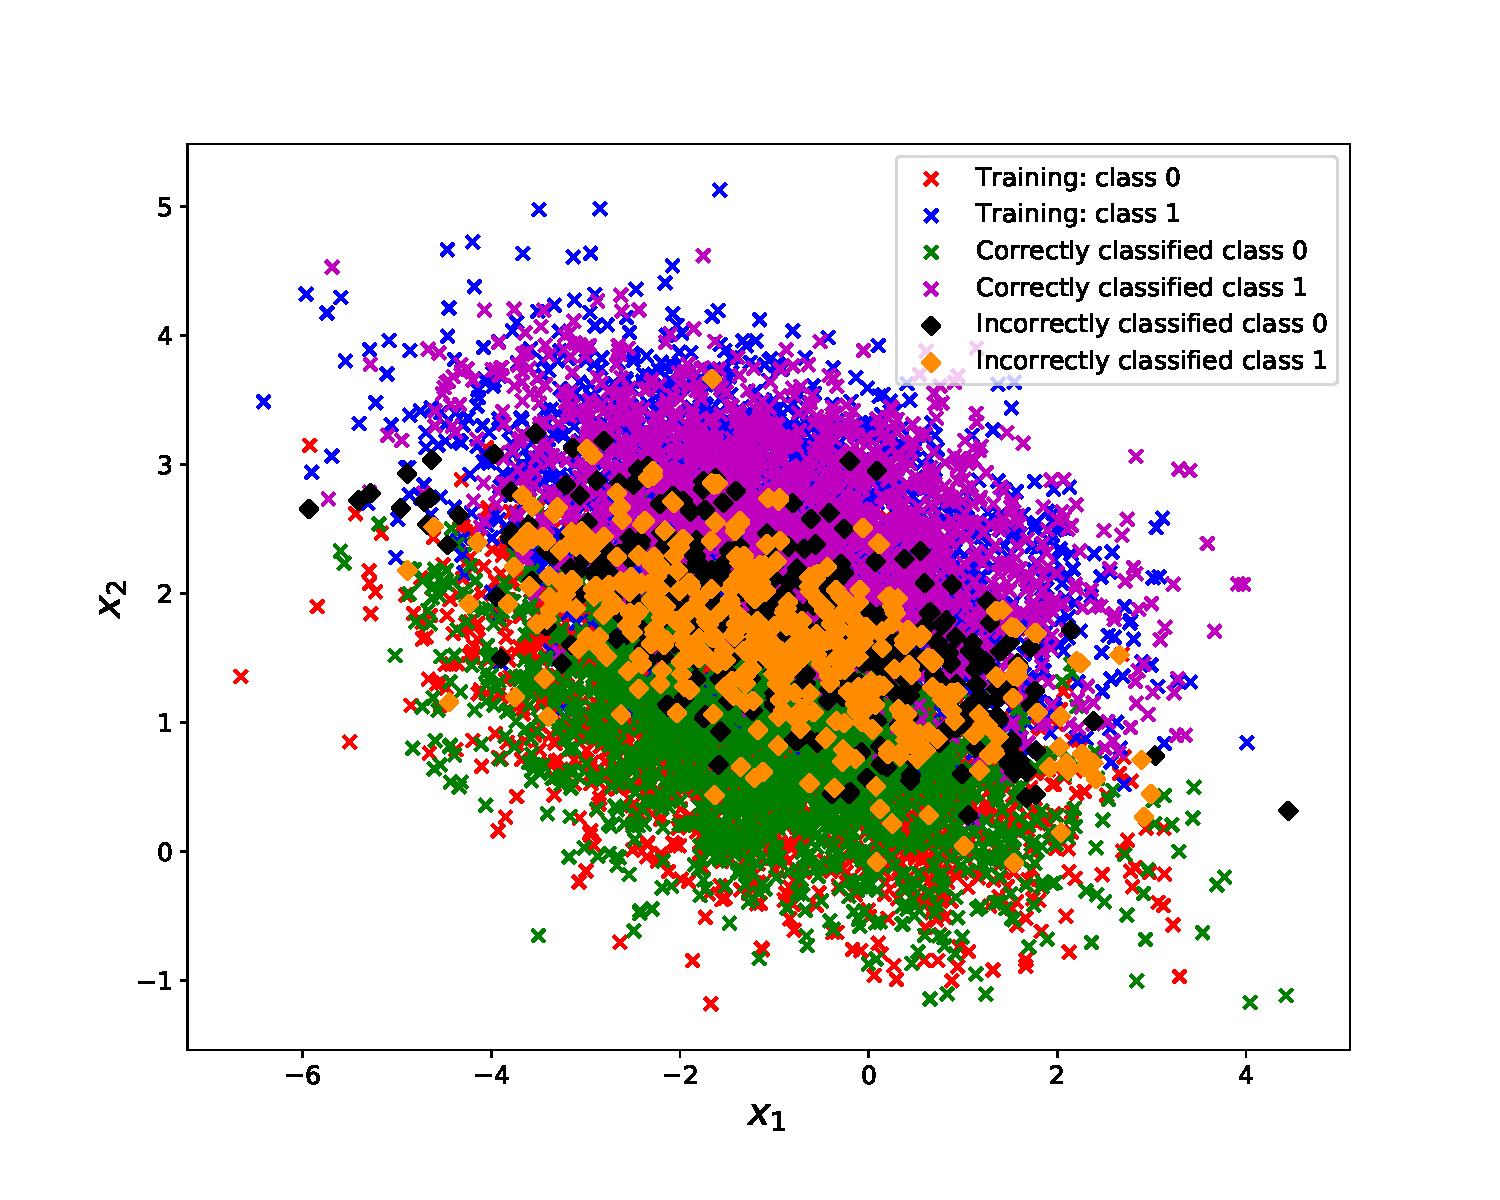
\includegraphics[width=0.8\textwidth]{figures/kdtree_classifier.pdf}}
\caption{The data is generated from two different multivariate Gaussian distribution and is split into train and test data with 50\%. $k$D tree classifier achieves accuracy of \underline{\textbf{82.32\%}} on test data.}
\label{fig:kdtree_classifier_1}
\end{figure*}

\newpage
\section{Increasing complexity}
\begin{figure*}[htbp]
\centering
{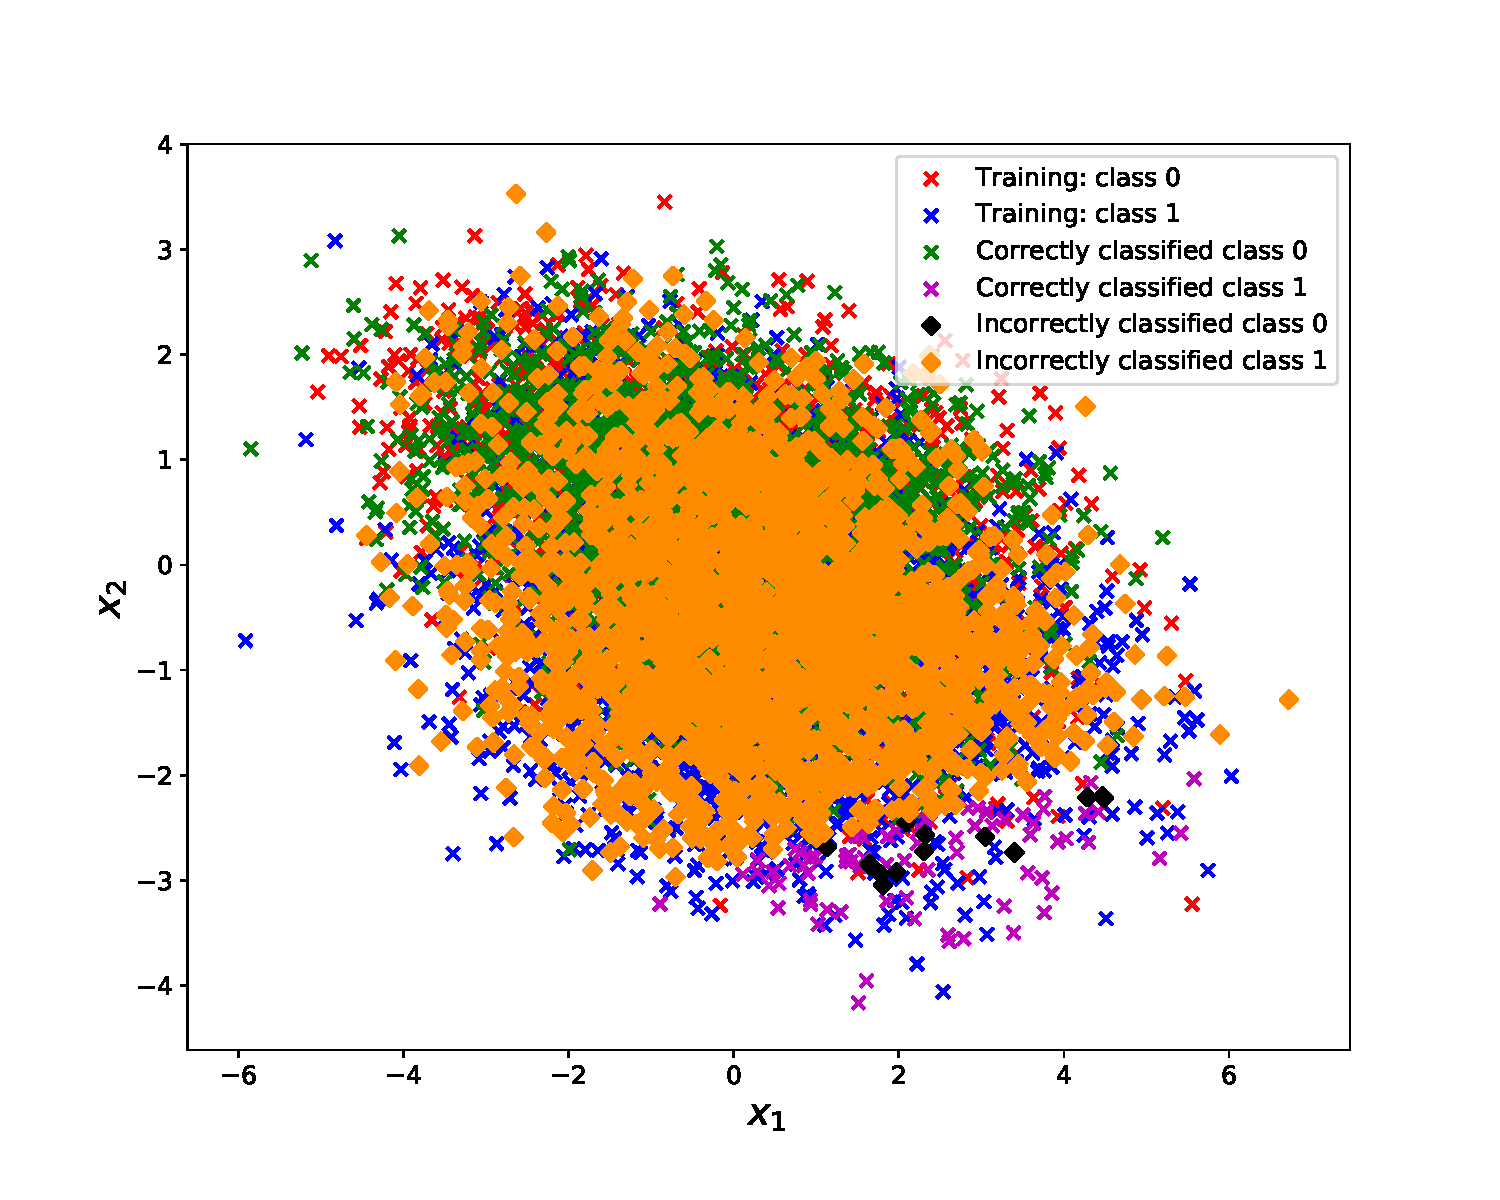
\includegraphics[width=0.8\textwidth]{figures/linear_classifier_5.pdf}}
\caption{The data is generated from ten different multivariate Gaussian distribution and is split into train and test data with 50\%. Five of them are assigned label 0 and the others 1. Linear classifier achieves accuracy of \underline{\textbf{51.2\%}} on test data.}
\label{fig:lin_classifier_5}
\end{figure*}

\begin{figure*}[htbp]
\centering
{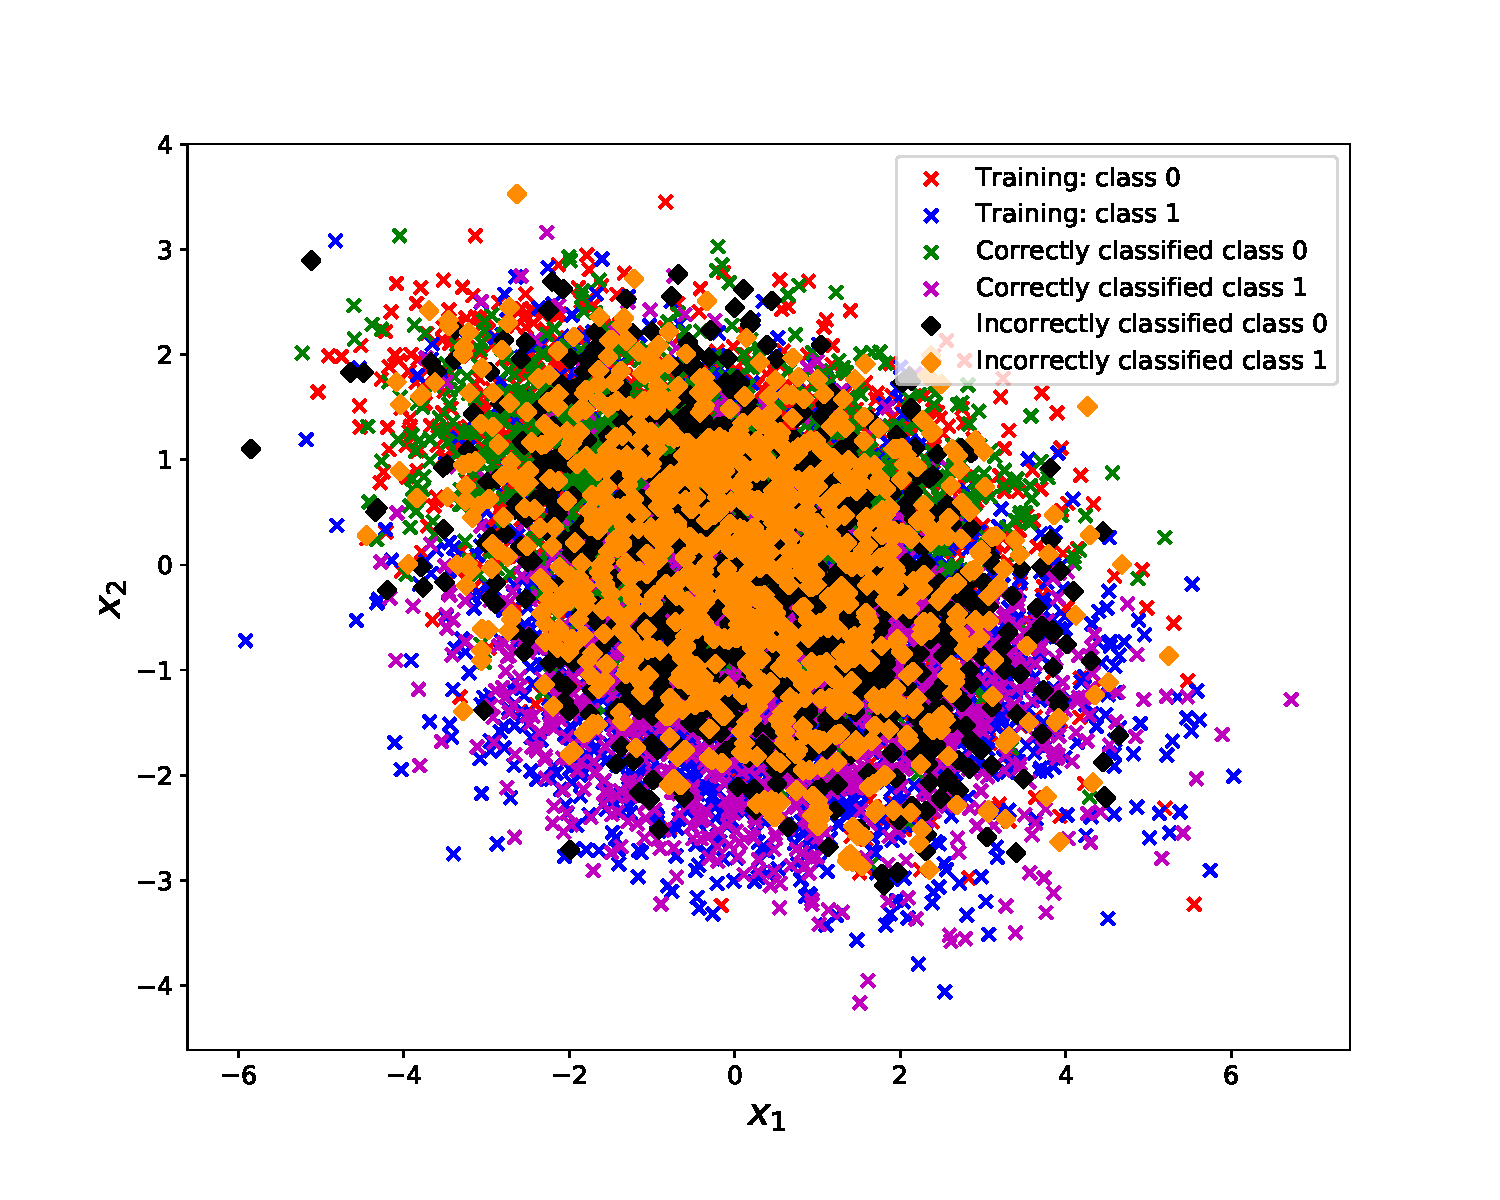
\includegraphics[width=0.8\textwidth]{figures/kdtree_classifier_5.pdf}}
\caption{The data is generated from ten different multivariate Gaussian distribution and is split into train and test data with 50\%. Five of them are assigned label 0 and the others 1. $k$D tree classifier achieves accuracy of \underline{\textbf{57.84\%}} on test data.}
\label{fig:kdtree_classifier_5}
\end{figure*}

\end{document}
